% !TEX TS-program = pdflatex
% !TEX encoding = UTF-8 Unicode

% This is a simple template for a LaTeX document using the "article" class.
% See "book", "report", "letter" for other types of document.

\documentclass[11pt]{article} % use larger type; default would be 10pt
\hbadness=10000
\usepackage{amssymb,amsmath}
\usepackage[utf8]{inputenc} % set input encoding (not needed with XeLaTeX)
%%% Examples of Article customizations
% These packages are optional, depending whether you want the features they provide.
% See the LaTeX Companion or other references for full information.
\newcommand{\ud}{\, \text{d}}
%%% PAGE DIMENSIONS
\usepackage{geometry} % to change the page dimensions
\geometry{a4paper} % or letterpaper (US) or a5paper or....
% \geometry{margin=2in} % for example, change the margins to 2 inches all round
% \geometry{landscape} % set up the page for landscape
%   read geometry.pdf for detailed page layout information

\usepackage[pdftex]{graphicx}
\usepackage[colorlinks, linkcolor=red, anchorcolor=purple, citecolor=blue]{hyperref}
\usepackage{epstopdf} % support the \includegraphics command and options

% \usepackage[parfill]{parskip} % Activate to begin paragraphs with an empty line rather than an indent

%%% PACKAGES
\usepackage{pgf}
\usepackage{tikz}
\usetikzlibrary{arrows}
\usepackage{booktabs} % for much better looking tables
\usepackage{array} % for better arrays (eg matrices) in maths
\usepackage{paralist} % very flexible & customisable lists (eg. enumerate/itemize, etc.)
\usepackage{verbatim} % adds environment for commenting out blocks of text & for better verbatim
\usepackage{float}
\usepackage{subfig} % make it possible to include more than one captioned figure/table in a single float
% These packages are all incorporated in the memoir class to one degree or another...
\usepackage{ulem}
\usepackage{color}


%%% HEADERS & FOOTERS
\usepackage{fancyhdr} % This should be set AFTER setting up the page geometry
\pagestyle{fancy} % options: empty , plain , fancy
\renewcommand{\headrulewidth}{0pt} % customise the layout...
\lhead{}\chead{}\rhead{}
\lfoot{}\cfoot{\thepage}\rfoot{}

%%% SECTION TITLE APPEARANCE
\usepackage{sectsty}
\allsectionsfont{\sffamily\mdseries\upshape} % (See the fntguide.pdf for font help)
% (This matches ConTeXt defaults)

%%% ToC (table of contents) APPEARANCE
\usepackage[nottoc,notlof,notlot]{tocbibind} % Put the bibliography in the ToC
\usepackage[titles,subfigure]{tocloft} % Alter the style of the Table of Contents
\renewcommand{\cftsecfont}{\rmfamily\mdseries\upshape}
\renewcommand{\cftsecpagefont}{\rmfamily\mdseries\upshape} % No bold!

%%%From Allan
% Math commands by Thomas Minka

\newcommand{\var}{{\rm var}}

\newcommand{\Tr}{^{\rm T}}

\newcommand{\vtrans}[2]{{#1}^{(#2)}}

\newcommand{\kron}{\otimes}

\newcommand{\schur}[2]{({#1} | {#2})}

\newcommand{\schurdet}[2]{\left| ({#1} | {#2}) \right|}

\newcommand{\had}{\circ}

\newcommand{\diag}{{\rm diag}}

\newcommand{\invdiag}{\diag^{-1}}

\newcommand{\rank}{{\rm rank}}

% careful: ``null'' is already a latex command

\newcommand{\nullsp}{{\rm null}}

\newcommand{\tr}{{\rm tr}}

\renewcommand{\vec}{{\rm vec}}

\newcommand{\vech}{{\rm vech}}

\renewcommand{\det}[1]{\left| #1 \right|}

\newcommand{\pdet}[1]{\left| #1 \right|_{+}}

\newcommand{\pinv}[1]{#1^{+}}

\newcommand{\erf}{{\rm erf}}

\newcommand{\hypergeom}[2]{{}_{#1}F_{#2}}



% boldface characters

\renewcommand{\a}{{\bf a}}

\renewcommand{\b}{{\bf b}}

\renewcommand{\c}{{\bf c}}

\renewcommand{\d}{{\rm d}}  % for derivatives

\newcommand{\e}{{\bf e}}

\newcommand{\f}{{\bf f}}

\newcommand{\g}{{\bf g}}

\newcommand{\h}{{\bf h}}

%\newcommand{\k}{{\bf k}}

% in Latex2e this must be renewcommand

\renewcommand{\k}{{\bf k}}

\newcommand{\m}{{\bf m}}

\newcommand{\n}{{\bf n}}

\renewcommand{\o}{{\bf o}}

\newcommand{\p}{{\bf p}}

\newcommand{\q}{{\bf q}}

\renewcommand{\r}{{\bf r}}

\newcommand{\s}{{\bf s}}

\renewcommand{\t}{{\bf t}}

\renewcommand{\u}{{\bf u}}

\renewcommand{\v}{{\bf v}}

\newcommand{\w}{{\bf w}}

\newcommand{\x}{{\bf x}}

\newcommand{\y}{{\bf y}}

\newcommand{\z}{{\bf z}}

\newcommand{\A}{{\bf A}}

\newcommand{\B}{{\bf B}}

\newcommand{\C}{{\bf C}}

\newcommand{\D}{{\bf D}}

\newcommand{\E}{{\bf E}}

\newcommand{\F}{{\bf F}}

\newcommand{\G}{{\bf G}}

\renewcommand{\H}{{\bf H}}

\newcommand{\I}{{\bf I}}

\newcommand{\J}{{\bf J}}

\newcommand{\K}{{\bf K}}

\renewcommand{\L}{{\bf L}}

\newcommand{\M}{{\bf M}}

\newcommand{\N}{{\cal N}}  % for normal density

%\newcommand{\N}{{\bf N}}

\renewcommand{\O}{{\bf O}}

\renewcommand{\P}{{\bf P}}

\newcommand{\Q}{{\bf Q}}

\newcommand{\R}{{\bf R}}

\renewcommand{\S}{{\bf S}}

\newcommand{\T}{{\bf T}}

\newcommand{\U}{{\bf U}}

\newcommand{\V}{{\bf V}}

\newcommand{\W}{{\bf W}}

\newcommand{\X}{{\bf X}}

\newcommand{\Y}{{\bf Y}}

\newcommand{\Z}{{\bf Z}}



% this is for latex 2.09

% unfortunately, the result is slanted - use Latex2e instead

%\newcommand{\bfLambda}{\mbox{\boldmath$\Lambda$}}

% this is for Latex2e

\newcommand{\bfLambda}{\boldsymbol{\Lambda}}



% Yuan Qi's boldsymbol

\newcommand{\bsigma}{\boldsymbol{\sigma}}

\newcommand{\balpha}{\boldsymbol{\alpha}}

\newcommand{\bpsi}{\boldsymbol{\psi}}

\newcommand{\bphi}{\boldsymbol{\phi}}

\newcommand{\bPhi}{\boldsymbol{\Phi}}

\newcommand{\bbeta}{\boldsymbol{\beta}}

\newcommand{\Beta}{\boldsymbol{\eta}}

\newcommand{\btau}{\boldsymbol{\tau}}

\newcommand{\bvarphi}{\boldsymbol{\varphi}}

\newcommand{\bzeta}{\boldsymbol{\zeta}}



\newcommand{\blambda}{\boldsymbol{\lambda}}

\newcommand{\bLambda}{\mathbf{\Lambda}}



\newcommand{\btheta}{\boldsymbol{\theta}}

\newcommand{\bpi}{\boldsymbol{\pi}}

\newcommand{\bxi}{\boldsymbol{\xi}}

\newcommand{\bSigma}{\boldsymbol{\Sigma}}



\newcommand{\bgamma}{\mathbf{\gamma}}

\newcommand{\bGamma}{\mathbf{\Gamma}}



\newcommand{\brho}{\boldsymbol{\rho}}

\newcommand{\bmu}{\boldsymbol{\mu}}

\newcommand{\1}{{\bf 1}}

\newcommand{\0}{{\bf 0}}

\newcommand{\bs}{\backslash}

\newcommand{\ben}{\begin{enumerate}}

\newcommand{\een}{\end{enumerate}}



 \newcommand{\notS}{{\backslash S}}

 \newcommand{\nots}{{\backslash s}}

 \newcommand{\noti}{{\backslash i}}

 \newcommand{\notj}{{\backslash j}}

 \newcommand{\nott}{\backslash t}

 \newcommand{\notone}{{\backslash 1}}

 \newcommand{\nottp}{\backslash t+1}

% \newcommand{\notz}{\backslash z}



\newcommand{\notk}{{^{\backslash k}}}

%\newcommand{\noti}{{^{\backslash i}}}

\newcommand{\notij}{{^{\backslash i,j}}}

\newcommand{\notg}{{^{\backslash g}}}

\newcommand{\wnoti}{{_{\w}^{\backslash i}}}

\newcommand{\wnotg}{{_{\w}^{\backslash g}}}

\newcommand{\vnotij}{{_{\v}^{\backslash i,j}}}

\newcommand{\vnotg}{{_{\v}^{\backslash g}}}

\newcommand{\half}{\frac{1}{2}}

\newcommand{\msgb}{m_{t \leftarrow t+1}}

\newcommand{\msgf}{m_{t \rightarrow t+1}}

\newcommand{\msgfp}{m_{t-1 \rightarrow t}}



\newcommand{\proj}[1]{{\rm proj}\negmedspace\left[#1\right]}

\newcommand{\argmin}{\operatornamewithlimits{argmin}}

\newcommand{\argmax}{\operatornamewithlimits{argmax}}
\newcommand{\bbm}{\begin{bmatrix}}
\newcommand{\ebm}{\end{bmatrix}}

\newcommand{\dif}{\mathrm{d}}

\newcommand{\abs}[1]{\lvert#1\rvert}

\newcommand{\norm}[1]{\lVert#1\rVert}
%%%

%%% END Article customizations

%%% The "real" document content comes below...

\title{Summary 1 of Yelp Challenge 2014}
\author{Xiao (Cosmo) Zhang}
\date{\today} % Activate to display a given date or no date (if empty),
         % otherwise the current date is printed 

\begin{document}
\maketitle
\tableofcontents

\newpage
\section{Introduction}
All the basic information of the Yelp challenge 2014 can be found on this website: \url{http://www.yelp.com/dataset_challenge}

\section{Influential Social network}
Figure \ref{grh} shows a small fraction of a imaginary social network that can be restored from the Yelp dataset. The nodes are represent people in the network, while solid lines between two nodes indicate that they are friends. \sout{We here propose a research topic is related to the prediction of a user's rating of one business, by using the information of this influential social network.} We are interested in understanding the influence of social network on how a user rate a business. A influential social network is defined as the social network where two nodes are influencing each others attitude and formation of opinion towards certain objects. (ref here)
\begin{figure}[htb!]
\centering
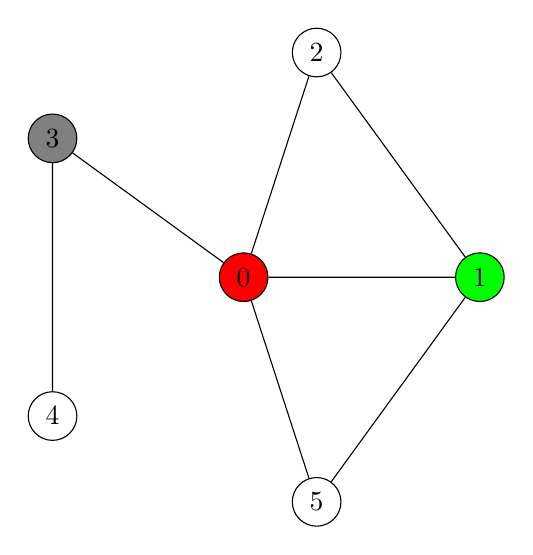
\begin{tikzpicture}
\tikzstyle{every node}=[draw,shape=circle];
\node [fill=red](v0) at (0:0) {$0$};
\node [fill=green](v1) at (0:3) {$1$};
\node (v2) at ( 72:3) {$2$};
\node [fill=gray](v3) at (2*72:3) {$3$};
\node (v4) at (3*72:3) {$4$};
\node (v5) at (4*72:3) {$5$};
\draw (v0) -- (v1)
	  (v1) -- (v2)
	  (v0) -- (v3)
	  (v3) -- (v4)
  	  (v0) -- (v5)
  	  (v0) -- (v2)
  	  (v1) -- (v5);
\end{tikzpicture}
\caption{An Illustration Graph}
\label{grh}	
\end{figure}

For example, in Figure \ref{grh}, node 1 and node 0 are influencing each other on a certain business, and so are node 0 and node 3 \sout{as well}. Suppose we are trying to predict the rating of node 0 on a certain business, and we \sout{are taking} take into consideration all the influences from his friends\sout{, and then} i.e. all the four nodes, 1, 2, 3, and 5 will have an effect on him. We believe that friends' rating of a certain business will have an impact on an individual's \sout{making of} decision of rating, but weighted according to the strength of influence each friend \sout{with different weights of different friends}. Hereby we currently propose three different perspectives that may strongly be related with the weights of the influence of a friend's rating on \sout{this} an individual: they are the \textbf{the number of common friends}, \textbf{the similarity of this individual and the friend}, and \textbf{the persuasive style of the friend} (ref)

\subsection{The number of common friends}
We believe that the more common friends two people have, the higher is the chance that these two people are within a same cluster, which implies that these two people are having a \sout{deeper} stronger relationship. In this case, a friend of this type may have a stronger influence on the individual. For instance. in Figure \ref{grh}, node 0, 1, 2, and 5 form a \sout{small} cluster, and node 0 and node 1 have two common friends, while node 0 and node 3 have no common friends. In this case, we assume node 1 will have a stronger influence on node 0 {\color{red} example seems incomplete}. Here we denote the number of common friends by $ a $.\\

$ a $ can be found by first forming a adjacency linked list. However, since a naive algorithm going through all the two pairs needs $ \binom{n}{2}=O(n^{2}) $ time, and find all the common friends of a pair will also consume $ O(n^{2}) $ time, a total of $ O(n^{4}) $ time will be need to perform this task. Therefore, transforming it into a adjacent matrix may bring some smart algorithm to reduce the time complexity.

\subsection{The persuasive style of the friend}
We believe different persuasive styles of an individual's friends will also have different weights on the decision making. For example, in Figure	\ref{grh}, the gray color of node 3 means node 3 is a very persuasive person, and likes give comments to things. In this case, apparently from this perspective node 3 will have a stronger influence on node 0 {\color{red} needs paraphrasing}. We denote the \textit{persuasive style} of the friend by $ b $, whose value is high if the friend is more persuasive.\\

We depict \sout{try to dig} the persuasive style of the friend by using two methods, one is just the number of comments (or words of comments) he gave, which is denoted by $ w $; the other is by mining the review text of a person, we try to identify his persuasive personality, which is denoted by $ v $. \sout{By doing a mining in the text of review,} To mine the review text, we might need some reliable NPL (Natural Language Processing) tools. Therefore, we can denote $ b $ as a function of $ w $ and $ v $ i.e. ($ b=g(w,v) $).

\subsection{The similarity of this individual and the friend}
We use $ c $ to denote the similarity between two nodes. We assume, if two people have a high similarity, they will focus on similar topics and elements of the business, and be interested in similar aspects of a business. $ c $ can be obtained by using a inner product of two vectors as $ c=\zeta_{1} \Tr\zeta_{2} $, if we use a vector $ \zeta $ to represent the properties of a node. (ref)\\

Then our task will be how to identify the properties of a node. We propose that the properties are hidden topics in the review comments. Therefore, a LDA (Latent Dirichlet allocation) model will be extremely useful to mine the hidden topics from the review text. Or maybe Collaborative Filtering will also be useful.

\section{Modeling}
We can buid the model in this way: First we propose $ \beta_{i}=H(a_{i}, b_{i}, c_{i}) $, \sout{give $ a $, $ b $, and $ c $, which is} as the weight function of the individual's $ i $th friend. Also, if we consider the trade-off effect, we can wrtie $ \beta_{i}=H(a_{i}+(1-\alpha_{1})b_{i}+(1-\alpha_{2})c_{i}) $, where $ \alpha_{1} $ and $ \alpha_{2} $ are importance coefficients. Then we can construct a regression model: $$ y= J(\sum\limits_{i}\beta_{i}x_{i})=J(\bbeta\Tr\x)$$, where $ \x $ is his friend's ratings on a certain business, $ \bbeta $ is the influential weights of his friends as a vector, and $ y $ is the rating of prediction. \sout{Here we consider} A multinomial logit regression, or a multinomial probit regression will be a good choice, because the output $ y $ is both discrete and ordinal.

\section{Conclusion}
We have already constructed the linked list. And next step we are trying to see how many common business people have ratings in this network.


\bibliographystyle{plainnat}
\bibliography{all}

\end{document}